\documentclass[12pt]{beamer} 
\usepackage{times}
\usepackage[]{algorithm2e}
%\SetKw{def}{def}
%\SetKw{To}{to} 
%\SetKw{Othera}{other}
%\SetKw{Become}{become}

\usepackage[T1]{fontenc} % bedre orddeling og ofte påkrævet at
\usepackage[utf8]{inputenc} % eller utf8 eller ansinew eller ...
\usepackage[english, danish]{babel} %direktiv til at bruge det danske sprog
\usepackage{graphicx} % pakke til inklusion af grafik
 
\renewcommand\danishhyphenmins{22} % bedre orddeling
\addto\captionsdanish{
\renewcommand\contentsname{Indholdsfortegnelse}
\renewcommand\appendixname{Appendix}
}
\selectlanguage{danish}
 
\usepackage[]{booktabs}
\usepackage{listings}
 \lstset{ 
         basicstyle=\tiny\ttfamily, % Standardschrift
         numbers=left,               % Ort der Zeilennummern
         numberstyle=\tiny,          % Stil der Zeilennummern
         stepnumber=2,               % Abstand zwischen den Zeilennummern
         numbersep=5pt,              % Abstand der Nummern zum Text
         tabsize=2,                  % Groesse von Tabs
         extendedchars=true,         %
         breaklines=false,            % Zeilen werden Umgebrochen
         keywordstyle=\color{red},
                frame=b,         
         keywordstyle=[1]\textbf,    % Stil der Keywords
         keywordstyle=[2]\textbf,    %
         keywordstyle=[3]\textbf,    %
         keywordstyle=[4]\textbf,   %\sqrt{\sqrt{}} %
         stringstyle=\color{black}\ttfamily, % Farbe der String
         showspaces=false,           % Leerzeichen anzeigen ?
         showtabs=false,             % Tabs anzeigen ?
         xleftmargin=17pt,
         framexleftmargin=17pt,
         framexrightmargin=5pt,
         framexbottommargin=4pt,
         %backgroundcolor=\color{lightgray},
         showstringspaces=false      % Leerzeichen in Strings anzeigen ?        
 }

 \lstloadlanguages{% Check Dokumentation for further languages ...
         [Visual]Basic,
         Pascal,
         C,
         C++,
         XML,
         HTML,
         PYTHON,
 }
\lstset{language=Python}
\lstset{emph={@process, @choise,choice, Alternation, Skip,Timeout,Parallel,Sequence, Spawn,@io,ChannelPoisonException, ChannelRetireException},emphstyle=\underbar}

\newcommand\mc[1]{\multicolumn{1}{c}{\textbf {#1}}} % sparer plads


% A few keywords to use in pseudocode
% You should also probably read the algorithm2e -documentation more than I did.

\usetheme[nat,dk,style=simple]{Frederiksberg}% Beamer theme v 3.0
%\mode<presentation>
%{
%\usetheme{Rochester}% Beamer theme v 3.0
%\usecolortheme{whale}
%   \setbeamercovered{transparent}
%   \definecolor{beamer@tkkblue}{HTML}{0041AD}
%   \setbeamercolor{structure}{fg=beamer@tkkblue}
%} 
\title
{Timed PyCSP}
%\subtitle
%{Specialeforsvar}
\institute
{Datalogisk Institut \\ Københavns Universitet}
\author
{Simon Bognolo}
\date
{5 juli 2010}


\begin{document}

\frame[plain]\titlepage
 
\begin{frame}
  \frametitle{Oversigt}
  \tableofcontents
\end{frame}

\section{Formål}
\begin{frame}
  \frametitle{Formålet med dette speciale er:}
  \begin{itemize}
	\item Praktisk anvendelig implementering af tid i PyCSP
	\item Ensartet håndtering af tid i PyCSP
	\item Let at anvende
  \end{itemize}
\end{frame}

 
\section{PyCSP}
\begin{frame} [fragile]
  \frametitle{Scheduleren i PyCSP}
  \begin{itemize}
	\item Er en brugertråd
	\item Har ingen tvungen kontekstskift
	\item Har introduceret tid via Timeouts
  \end{itemize}
\begin{lstlisting}
Alternation([{Timeout(seconds=0.5):None}, {Cin:None}]).select()
\end{lstlisting}
\end{frame}

\begin{frame}
  \frametitle{Gennemgang af scheduleren}
  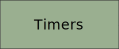
\includegraphics[scale=0.9]{pycsp-scheduler} 
\end{frame}

\section{Simulering i diskret tid (DES)}
\begin{frame}
  \frametitle{Simulering i diskret tid (DES)\\
-  Simulering af Minimum Intrusion Grid
}
  \includegraphics[scale=0.3]{mig}  
\end{frame}

\begin{frame}
  \frametitle{Simulation af Minimum Intrusion Grid
}
  \includegraphics[scale=0.45]{tidsmodel-1}
  \includegraphics[scale=0.45]{queue}
\end{frame}


%\begin{frame}
%\frametitle{Implementering}
%  \begin{itemize}   
%	\item Udvide scheduler
%	%\item Håndtering af køer
%  \end{itemize}
%\end{frame}
 
\begin{frame}
\frametitle{Udvidelsen af scheduleren}
\includegraphics[scale=0.9]{des-scheduler} 
\end{frame}


\section{Real-time planlægning (RTP)}
\begin{frame}
  \frametitle{Real-time planlægning (RTP)}
\includegraphics[scale=0.35]{Process_Model_GUI} 
\end{frame}

\begin{frame}
  \frametitle{Real-time planlægning (RTP)}
  \begin{itemize}
	\item Udvidelse af processer:
	  \begin{itemize}   
		\item Deadline
		\item Bruger prioritet
		\item Beregnet prioritet	
		\item Nedarvet prioritet
	  \end{itemize}
	\item Udvidelse af kanaler:
	  \begin{itemize}   
		\item Tilknytte processer med kanalender
		\item Udvælger processer til kommunikation
	  \end{itemize}
\end{itemize}
\end{frame}


\begin{frame}
	\frametitle{RTP og PyCSP indvirkning på kommunikation ved}
	\begin{itemize}
		\item Any-to-Any Kanaler 
	 	\item Alternation
	\end{itemize} 
\begin{center}
	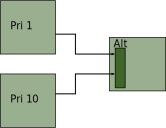
\includegraphics[scale=0.7]{alt-inheritance.pdf} 
\end{center}
\end{frame} 


\begin{frame}
  \frametitle{RTP scheduler}
\includegraphics[scale=0.9]{rtp-scheduler}
\end{frame}

\begin{frame}
  \frametitle{Prioritetsnedarvning}

\includegraphics[scale=0.7]{nedarvning} 
\end{frame}
\begin{frame}
  \frametitle{Prioritetsnedarvning}
\includegraphics[scale=0.7]{nedarvning2} 
\end{frame}
\begin{frame}
  \frametitle{Prioritetsnedarvning}
\includegraphics[scale=0.7]{nedarvning3} 
\end{frame}
\begin{frame}
  \frametitle{Prioritetsnedarvning}
\includegraphics[scale=0.7]{nedarvning4} 
\end{frame}
\begin{frame}
  \frametitle{Prioritetsnedarvning}
\includegraphics[scale=0.7]{nedarvning5} 
\end{frame}


%\subsection{Resultater}
%\begin{frame}
%  	\frametitle{RTP resultater}
%	\tiny 
%	\begin{table}[htbp]
%		\centering
%		\begin{tabular}{lcccc}
%		   	\toprule
%		    \mc{Version}&\mc{Tid i dummyproces(s)}&\mc{SA.}& \mc{Succesrate (\%)}&\mc{SA.}\\
%		    \midrule
%		    Greenlets         & 1.29 & 0.61 & 13 & 2  \\
%		    RTP u. prioritet  & 1.05 & 0.28 & 24 & 6  \\
%		    RTP m. prioritet  & 0.74 & 0.34 & 42 & 13 \\
%		    \bottomrule
%		\end{tabular}
%		\caption[]{\tiny 10 * 100 grise køres igennem procesnetværket. Samtidigt køres en dummyproces.}
%	\end{table}
%\end{frame} 

\section{Fremtidigt arbejde}
\begin{frame}
  	\frametitle{Fremtidigt arbejde}
\begin{itemize}
\item DES
	\begin{itemize}
	%\item Dynamisk køskifte
	%\item Reservering af flere ressurcer
	\item Stopkriterium
	\item Parallelisering
	\end{itemize}
\item RTP
	\begin{itemize}
	%\item Estimater for udførselstid
	\item Samarbejde med operativsystemet
	%\item Forskellige typer deadlines
	\end{itemize}
\end{itemize}
\end{frame}
 


\end{document}

 
